\documentclass[12pt]{article}

\usepackage{fullpage}
\usepackage{multicol,multirow}
\usepackage{tabularx}
\usepackage{listings}
\usepackage{pgfplots}
\usepackage[utf8]{inputenc}
\usepackage[russian]{babel}
\usepackage[T2A]{fontenc}
\usepackage{pgfplots}
\usepackage{tikz}


\begin{document}

% \newpage
% \begin{center}
% {\bfseries ФЕДЕРАЛЬНОЕ ГОСУДАРСТВЕННОЕ БЮДЖЕТНОЕ ОБРАЗОВАТЕЛЬНОЕ\\
% УЧРЕЖДЕНИЕ ВЫСШЕГО ОБРАЗОВАНИЯ\\
% «МОСКОВСКИЙ АВИАЦИОННЫЙ ИНСТИТУТ\\
% (НАЦИОНАЛЬНЫЙ ИССЛЕДОВАТЕЛЬСКИЙ УНИВЕРСИТЕТ)»}
% \vspace{1cm}

% Журнал лабораторных работ
% \vspace{6em}

% \vspace{\fill}

% \begin{center}
% Москва 2024
% \newpage
% \end{center}

\section*{Лабораторная работа №2\, по курсу компьютерной графики}

\textbf{Тема:} Основы 3D-графики и проекция\\
\\
\textbf{Задача:} Познакомится с основами 3D-графики: построением простых 3D-объектов, проекцией на 2D-плоскость, а также научиться работать с матрицами перспективы и ортографической проекции. \\
\\
\textbf{Вариант:} 2. Построение пирамиды с перспективной проекцией\\
Постройте 3D-пирамиду (с квадратным основанием).\\
Примените перспективную проекцию для отображения пирамиды.\\
Реализуйте вращение пирамиды вокруг всех осей с помощью клавиш управления.\\
Дополнительно: Добавьте динамическое изменение угла обзора (field of view) и наблюдайте, как это влияет на проекцию.\\


\subsection*{1 Решение}

Для выполнения этой лабораторной работы я использовал библиотеку SFML. Но так как она создана для работы с 2D-графикой, пришлось реализовывать перспективную проекцию. 
Я добавил функции вращения по всем осям. Саму пирамиду я представил в виде 5 точек, соеденённых линиями, и уже эти 5 точек я перемещал, для создания иллюзии 3D. Фокусное расстояние
по сути увеличивает размер фигуры по Z-координате, тоесть в сторону пользователя.

\begin{figure}[h]

    \centering
        
    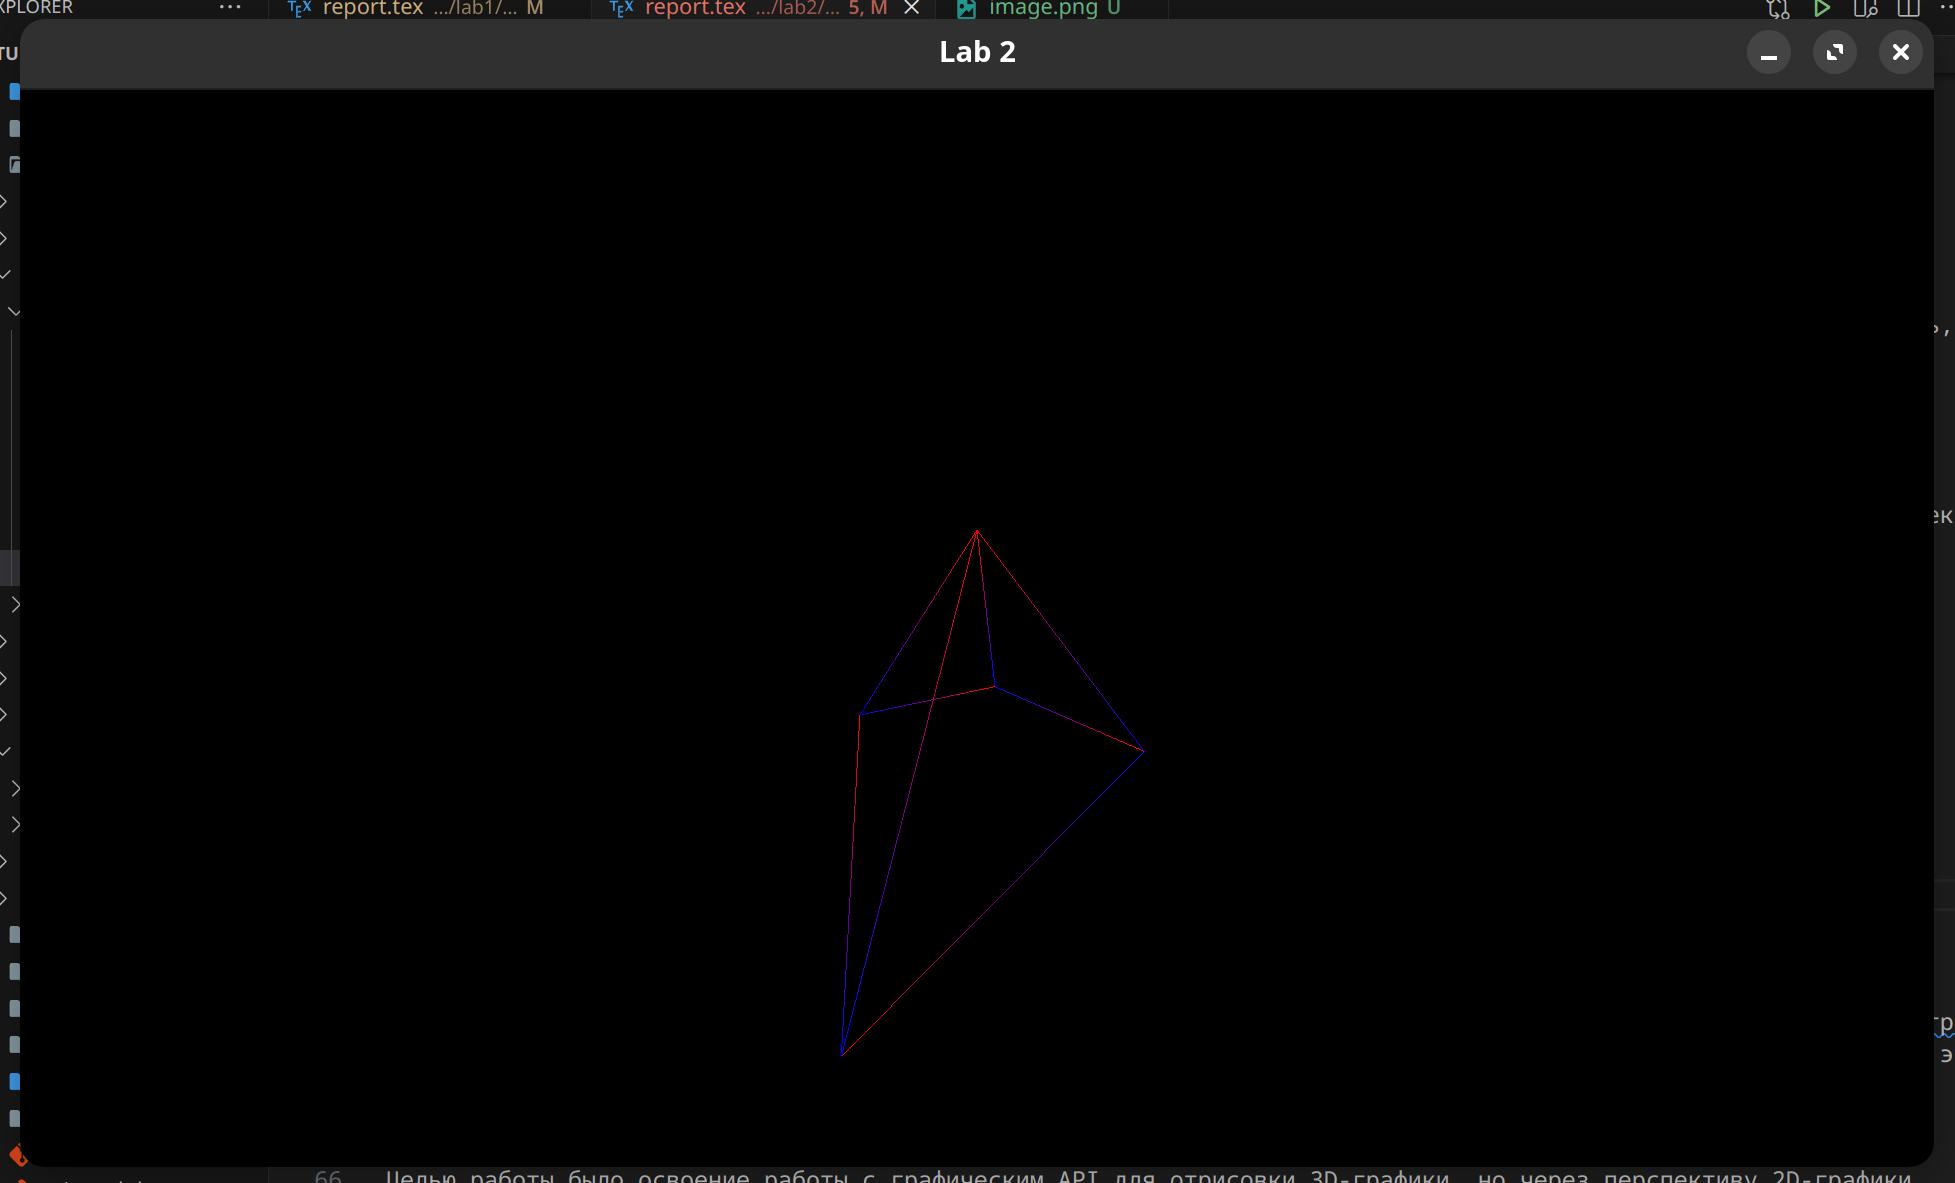
\includegraphics[width=0.8\linewidth]{image.png}
        
    \caption{Пример работы программы}
        
    \label{fig:mpr}
        
    \end{figure}
    
\subsection*{2 Вывод}

Целью работы было освоение работы с графическим API для отрисовки 3D-графики, но через перспективу 2D-графики.
В ходе выполнения лабораторной работы получилось понять, как строить 3D-графику, проекцией на плоскость. 
По итогу, выполненная работа позволила не только овладеть основными аспектами работы с созданием 3D-графики в библиотеке, которая может отрисовывать только 2D-графику, но и применить полученные знания на практике.
\end{document}
